% status: 0
% chapter: TBD

\title{Sentiment Analysis of Cancer Immunotherapy-Relevant Tweets}


\author{Darren Wright}
\affiliation{%
  \institution{Indiana University}
  \streetaddress{School of Informatics, Computing, and Engineering}
  \city{Bloomington} 
  \state{IN} 
  \postcode{47408}
  \country{USA}
}

\begin{abstract}
  Research and funding for precision medicine continues to increase as
  big data technologies increase the potential for addressing a
  patient's individual, unique medical needs.  Immunotherapy is a form
  of precision medicine that leverages a patient's immune system to
  fight cancer.  It is a promising alternative for treating cancers
  not responsive to traditional treatments, though it also poses the
  danger of harming non-cancerous cells.

  This paper discusses the development and results of Python code
  written to assess the sentiment of streaming tweets relevant to this
  topic to better understand the state of this field in real-time.
  The analytic pipeline resulting from this effort targets advancing
  improving real-time, topic-based social media analysis to establish
  a solid foundation for future research.
\end{abstract}

\maketitle

\section{Introduction}

\TODO{some technologies are mentioned but no citations are given}

Research and funding for precision medicine-based cancer treatments
using the patient's own immune system to improve treatment results
continues to grow.  In particular, the field referred to commonly as
cancer immunotherapy attracts medical professionals who treat cancers
that do not respond well to traditional treatments like chemotherapy,
radiation, and gamma knife.  While immunotherapy poses significant
risks, it provides hope to cancer patients with few or no treatment
alternatives~\cite{hopkins2017}.
	
Analysis of social media may benefit the advancement of this field by
leveraging real-time data to gain a more holistic look at the state of
this field beyond clinical trials and journal
articles~\cite{kaya2017}.  In an approach akin to crowd-sourcing, this
project is an initial foray into analyzing streaming Twitter data to
establish a method for later work.  This project provides insight into
the following: (1) geographical locations with the highest frequency
of immunotherapy-related tweets, (2) overall perception
(\emph{sentiment}) of cancer immunotherapy, and (3) suggestions for
future research and analysis.  The resulting code, written in Python
2.7.14, provides an analytic pipeline as depicted in
Figure~\ref{fig:pipeline} to execute sentiment analysis of real-time
Twitter data.

\begin{figure}[H]
\centering
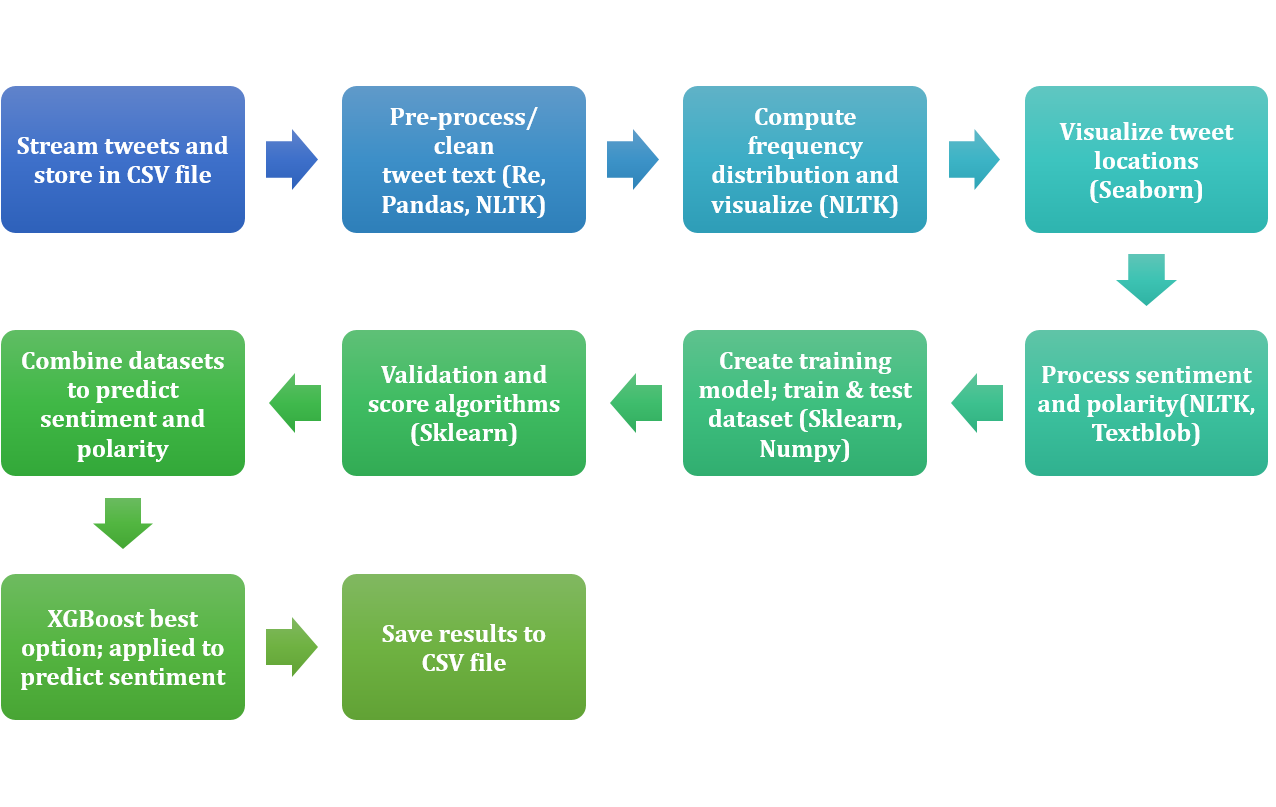
\includegraphics[width=\columnwidth]{images/sentiment_analysis_pipeline.png}
\caption{Overview of Sentiment Analysis Pipeline}
\label{fig:pipeline}
\end{figure}

\section{Data} 

To develop training and testing data sets for use
with a machine learning algorithm to predict
sentiment, 

\TODO{paper must not use the word I}

I developed two sets of data as follows:

\begin{itemize}
\item Train Data:  Natural Language Toolkit's
(\emph{NLTK}) Twitter sentiment corpus, which
provides two files:  one with positive tweets and one
with negative tweets formatted as shown in Figure 1.
These two files were used to create the training set
for the machine learning (ML) algorithm selected to
predict the sentiment for collected tweets~\cite{twitter14}.

\item Test Data:  Approximately 1,300 tweets collected via a
live-streaming Twitter feed.  These tweets were then partially
preprocessed while being saved as in CSV format for later usage.
\end{itemize}

\begin{figure}[H]
\centering
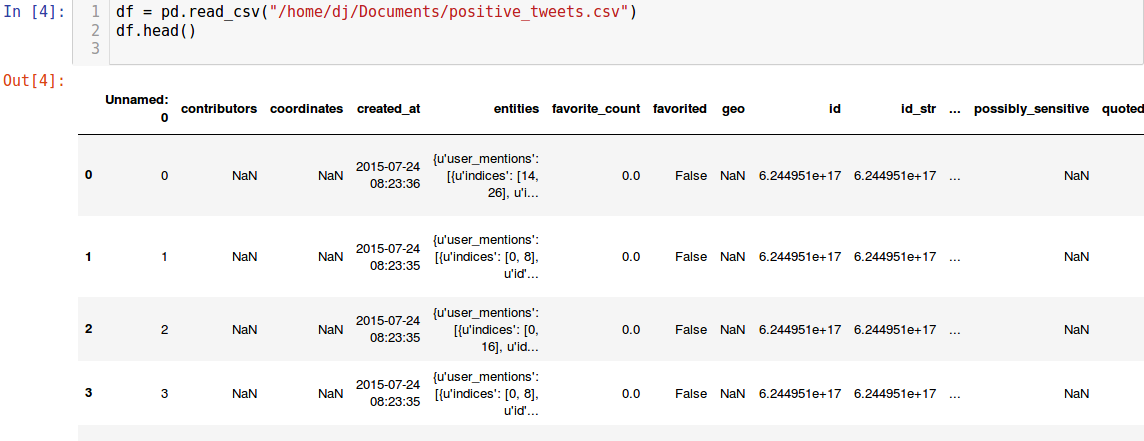
\includegraphics[width=\columnwidth]{images/screenshot_positive.png}
\caption{Positive Tweets file from NLTK}
\label{fig:positive}
\end{figure} 

For sentiment analysis, the code integrates NLTK's Twitter sentiment
corpora.  This corpora provides two files labeled
\verb|negative_tweets.json| and \verb|positive_tweets.json|.  As the
file names suggest, one file contains positive tweets and the other
negative tweets, but sentiment scores are not provided.  NLTK only
categorizes the tweets as positive or negatives based on the file they
belong to,sentiment and polarity scores were not provided.  Thus, each
of the three files were processed and formatted to contain three
columns -- sentence (\emph{tweet text}), polarity, and
sentiment~\cite{twitter_analysis}.

\begin{figure}[H]
\centering
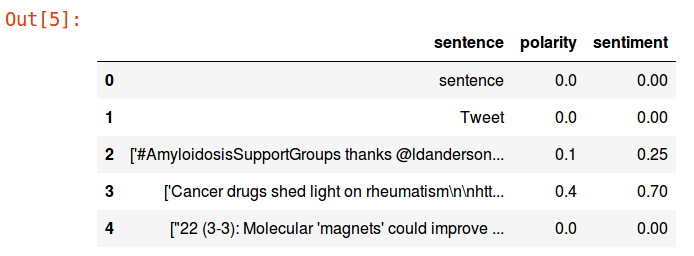
\includegraphics[width=\columnwidth]{images/collected_tweets_head.png}
\caption{Collected Tweets Processed Using TextBlob}
\label{fig:textblob_tweets}
\end{figure} 

\section{Methods}

Linking various packages to create a pipeline is difficult for
streaming a Twitter feed directly into a sentiment analysis pipeline.
This challenge is compounded by the numerous possible approaches to
choose from related to Python's main three packages for Twitter
streaming: Twitter, Tweepy, and Twython.  After multiple variations
were attempted to develop a code based on these three packages,
Twython was selected due to its flexibility and compatibility with
other packages like Pandas and
CSV~\cite{twitterU46,clay2013,python37,python-csv}.  This package is
the only one that provided solutions to the following critical issues:

\begin{itemize}
\item automatically breaking with the Twitter feed,
\item excluding all re-tweets,
\item allowing for multiple search terms
\item compatibility with the CSV package,
\item limiting the content saved from each tweet,
\item option to specify number of tweets and files.
\end{itemize}

Initial processing and visualization of the tweets was executed with
Python packages Re and NLTK.  NLTK's frequency distribution tool was
used to create the line chart in
Figure~\ref{fig:linechart,bird2016}.  This chart provides an
initial insight into potential themes and qualitative sentiment
associated with the topic of immunotherapy.  Interestingly, there are
no negative individual terms within the 40 most common words depicted
in the chart.

\begin{figure}[H]
\centering
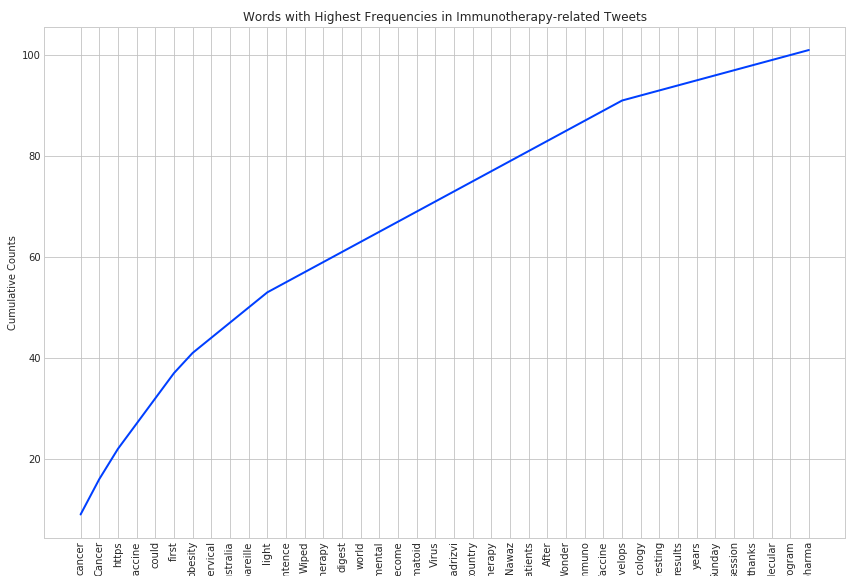
\includegraphics[width=\columnwidth]{images/linechart.png}
\caption{Tweet terms with highest frequencies}
\label{fig:linechart}
\end{figure} 

Seaborn~\cite{??} and Matplotlib.pyplot~\cite{??} were used to
visualize locations with the most tweets as shown in
Figure~\ref{fig:barchart}. Although this data sample is small,
previously collected at least 5000 tweets that also showed an
overwhelming majority of immunotherapy-related tweets originate from
the United States.  Europe and Australia also had a <significant
amount of tweets, though all other countries fell far short of these
three locations.  However, search terms in other languages like
Chinese, Japanese, and Arabic were not included.  This exclusion of
other languages likely significantly skews the data.

\begin{figure}[H]
\centering
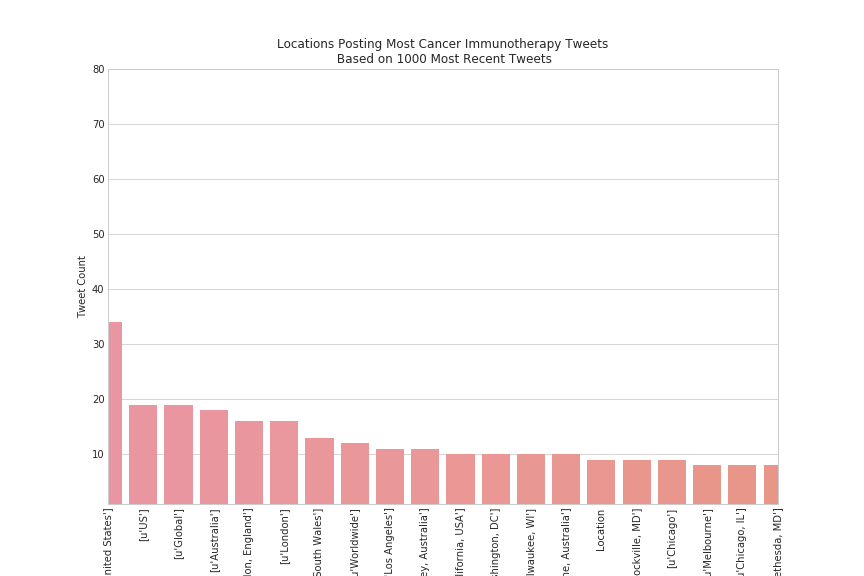
\includegraphics[width=\columnwidth]{images/barchart.png}
\caption{Locations with most immunotherapy-related tweets}
\label{fig:barchart}
\end{figure} 

Figure\ref{fig:sentline} also demonstrates the rather positive
sentiment toward immunotherapy.  As this figure illustrates, the
majority of tweets are of neutral sentiment, though there are several
small peaks on the positive side that outweigh the single peak on the
negative side of the chart.

\begin{figure}[H]
\centering
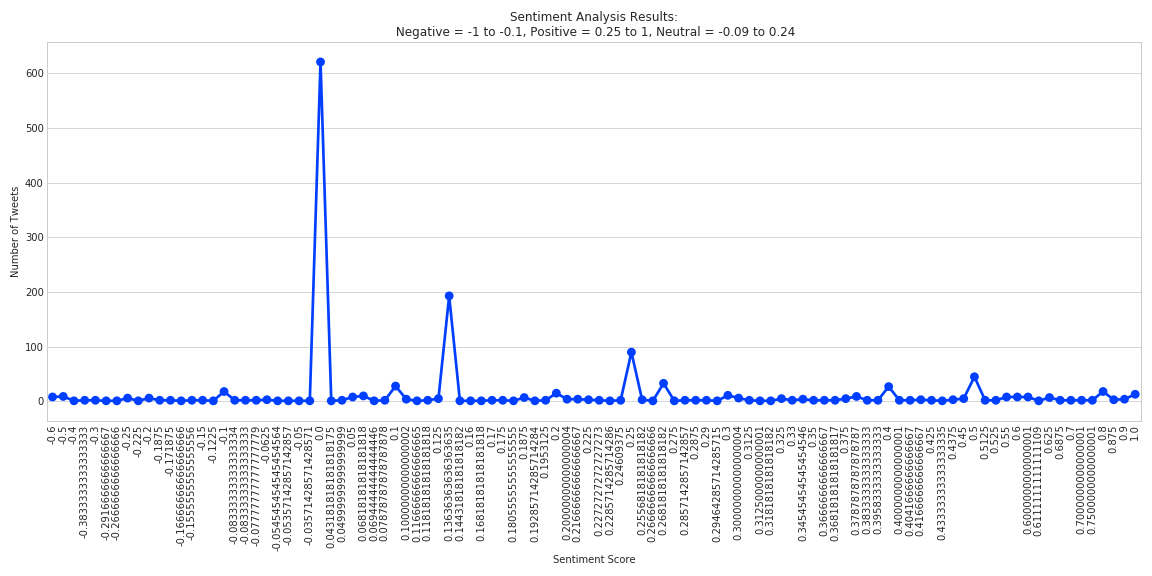
\includegraphics[width=\columnwidth]{images/sentiment_scores_linechart.png}
\caption{Locations with most immunotherapy-related tweets}
\label{fig:sentline}
\end{figure} 

Each file was then analyzed for sentiment using TextBlob, which
provided both sentiment and polarity scores (Figure 6).  Since NLTK
already provided a positive and negative file where sentiment had
already been assessed, TextBlob processing simply provided more
accurate scoring~\cite{jain2018}.  Sentiment analysis performed on the
collected tweets can be used later to compare this method with the
machine learning approach described later in this report.

Before settling on an algorithm to predict tweet sentiment, several
sub-modules from Sklearn were used cross-validation and accuracy
scoring for three different machine learning algorithms: naive Bayes,
support vector machine, and Sklearn's multi-layer perceptron (MLP)
neural
network~\cite{brownlee_2016,ads_algorithms,raschka2016}.

\begin{figure}[H]
\centering
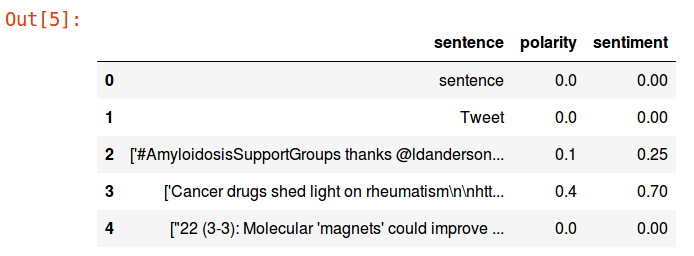
\includegraphics[width=\columnwidth]{images/collected_tweets_head.png}
\caption{Sentiment and Polarity Scores after TextBlob Processing}
\label{fig:scores_textblob}
\end{figure} 

\begin{figure}[H]
\centering
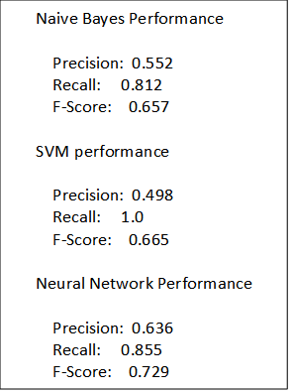
\includegraphics[width=\columnwidth]{images/ML_algorithms_performance.png}
\caption{Performance of Naive Bayes, Support Vector Machine, and
  Multi-Perceptron Neural Network}
\label{fig:performance_scores}
\end{figure} 

\section{Results}

The neural network algorithm performed the best out of the three
original algorithms considered for this project, which also included
Naive Bayes and Support Vector Machine.  Sklearn's neural network
algorithm resulted accuracy scores above 60 percent.  However, since
the desired score was 80\% or more, additional research posited the
Extreme Gradient Boosting (\emph{XGBoost}) algorithm as a likely
better candidate~\cite{Chen2016,baba2016,phunter2016}.
After testing this algorithm with the data and comparing the results
with the other three algorithms discussed above, it provided
significantly higher results with a top accuracy score of 76\%.

Since 2016, multiple Kaggle competition winners successfully applied
XGBoost along with Python’s Scikit-learn (\emph{Sklearn}) to improve
machine learning algorithms for processing disparate, sparse data.
Academic research further supports the utility of XGBoost as an
optimal approach to increasing the precision (the precision
(efficiency + accuracy) through more fully leveraging data and
handling imbalanced data.  The website Analytics Vidhya sums up the
advantages of using XGBoost as follows~\cite{jain2016}:

\begin{itemize}
\item reduces overfitting,
\item parallel processing through building parallel decision trees,
\item highly flexible, providing adjustable parameters for
  optimization and evaluation criteria,
\item handles missing values,
\item removes splits in the tree when they are no longer beneficial. 
\end{itemize}

Figure~\ref{F:output} shows one set of parameters used for XGBoost as
an example of just a few of the aspects of the algorithm the user can
adjust.

\begin{figure}[H]
\begin{verbatim}
  if diff:
[CV] ... learning_rate=0.3, max_depth=3, 
         score=0.751200 -  39.6s
[CV] learning_rate=0.3, max_depth=3 ...
\end{verbatim}
\caption{Top Accuracy Score Predicting Sentiment with XGBoost}\label{F:output}
\end{figure}

\begin{figure}[H]
\centering
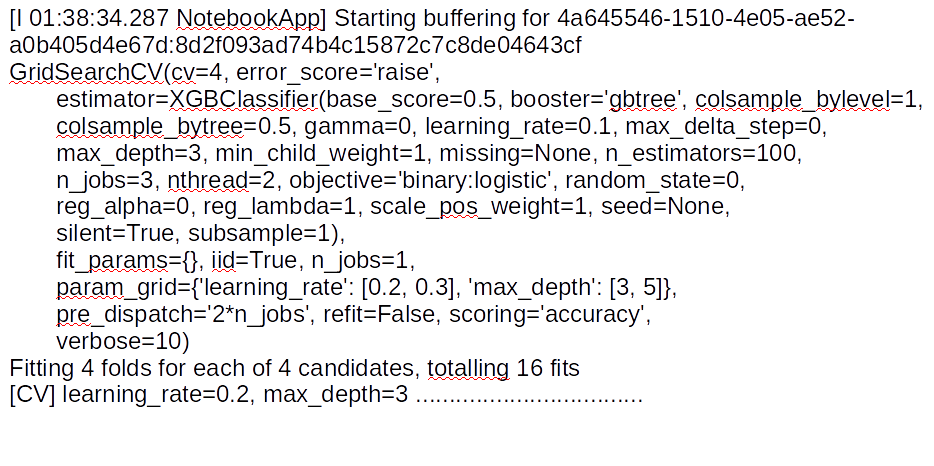
\includegraphics[width=\columnwidth]{images/xgb_params.png}
\caption{Example of XGBoost Parameters}
\label{fig:xgb_params}
\end{figure} 

Despite the relatively computationally intensive parameters selected
after several trials (Figure 5), XGBoost functioned without a hitch.
The program ran through 24 iterations of the code in as little as 20
minutes on a notebook computer, although the highest score was
achieved with a total runtime of 52 minutes.  The program ran on a
Dell Inspiron 7559 with the following specs:

\begin{itemize}
\item Intel Core 5th-generation i5-6300HQ (2.30GHz, quad-core)
\item Ubuntu 16.14 run on Oracle Virtual Box with Windows 10 as host
  system
\item 500GB Samsung SSD 850 EVO
\item NVidia GeForce 960M (4GB)
\end{itemize}

Access to multiple adjustable parameters proved beneficial.  One
parameter that made a significant difference is the \emph{nthread},
which defines the number of CPU cores used, significantly improved
accuracy and speed.  By increasing \emph{nthread}, used to adjust the
number of CPU cores used) from 1 to 4, the difference in computing
time for each of the folds went from around 5 to 8 minutes to between
30 and 45 sections each.  Despite using all 4 cores on the laptop,
other programs not memory-intensive ran without any major lag.
However, using 4 cores and increasing \emph{max\_depth} caused the
computer performance to drop significantly.

\section{Discussion}

This project aimed to create an easily executable program providing
insight for topic-based research through leveraging real-time,
streaming social media.  The resulting code allows for future
development of additional training and testing data sets as new data
becomes available.  The code also contains the following unique
characteristics:

\begin{itemize}
\item creates integrated pipeline for streaming,
storing, processing, visualizing, and saving
analysis in a single program; 
\item scalable as multiple search terms can be queried on separate virtual 
instances running the programming; 
\item decreases data bias by excluding re-tweets;
\item allows for flexible searches by allowing
user to use more than one search term;
\item executable in either Python 2.7 or 3+.
\end{itemize}

Overall, the analytic pipeline discussed in this report was successful
in achieving project goals.  Multiple issues related to streaming,
collecting, and storing tweets plaguing the first half of this project
were resolved.  Moreover, multiple packages and methods for analyzing
sentiment were integrated to make the pipeline more robust.  The
issues discussed later in this section outline some of the unique
challenges posed by open source programming, especially to newer
Python users.

Before discussing the issues, several data scientists who are generous
with sharing their work online along with open source Python
publications were critical in the success of this report
~\cite{sweigart2015,ojeda2014}.  Most significantly, Dr.\ Jason
Brownlee, the author of the website \emph{Machine Learning Mastery};
Brett Romero (\url{www.brettromero.com}); 

\TODO{NO URLS ALLOWED IN TEXT, MUST BE A CITATION}

and Tianqi Chen, the author of the XGB script benefited this project
from the micro level and on the macro level continue to contribute to
the international data science
community~\cite{brownlee_2016,romero2016,Chen2016}.

\emph{Challenges}: Significant issues, both expected and
unanticipated, appeared consistently throughout the course of
developing the code.  The lack of sufficient and useful approaches to
using Python for analyzing streaming Twitter or other social media
data was surprising, requiring me to spend a lot of time either
manipulating existing code or developing my own to accomplish were
seemingly simple tasks, including:

\begin{itemize}	
\item real-time processing and saving tweets to CSV-formatted files;
\item decreasing data bias by excluding re-tweets;
\item analyzing sentiment for newly collected
data;
\item converting tweet text to a binary format;
\item having the program break when a specified
number of tweets have been saved.
\end{itemize}

\begin{description}
\item[Python's rapid evolution:] Python and its packages evolve and/or
  become deprecated at a rapid pace.  This element of using Python as
  the programming language posed significant challenges throughout the
  course of completing this project.  Changes in code compatibility
  created difficulties.  Since the original code often worked when
  tested, it became very difficult to resolve problems that appeared
  as authors of the respective python package either changed or
  abandoned the package while other packages needed to complete the
  code became incompatible.

  \TODO{Instructors comments: you fail to mention the duration that
    you worked on this project. Python actually does not evolve much
    is has been mostly constant, but two versions exist 2.7 and
    3.6. This year most are transitioning to 3.6}

\item[Incompatibility of new Python packages:] Python 2.7+ is
  increasingly difficult to use to integrate updated or new packages.

  \TODO{Instructors comment: We provided class material on how to deal
    with thsi and switch between different python versions.}

  One frustrating instance arises from Python 2.7's handling of text
  encoding.  When using Textblob and Pandas to process tweets for
  sentiment, Python processed the text as ascii-encoded, but Textblob
  requires UTF-8.  Using Jupyter Notebook further compounded the issue
  because the simplest solution – using \verb|reload(sys)| and then
  setting the default encoding to \emph{utf-8}—caused the results of
  the code to print in the terminal window and not the notebook
  itself.  There is no resolution for this small, albeit very
  inconvenient, issue.
 
  \TODO{Instructors comment: python has a decode function and you can
    use utf-8, or converts it in a format you like. Also see python
    3.6}

\item[Useful test cases are scarce]: Many aspiring data scientists
  post or publish their knowledge of Python to collect and store,
  process, and visualize real-time streaming social media.  However,
  only after attempting to fit their techniques to real-life
  application for topic-based analysis did 
\TODO{I}
 discover that virtually
  none use data sets not already processed and structured for
  immediate use with machine learning algorithms.
\end{description}

As an example, one tutorial involves a drawn-out, but seemingly
promising, approach to conduct detailed sentiment analysis.  After an
extended period was spent figuring out why the model failed to work
after modifying the code repeatedly, it was discovered that the
pipeline used pre-processed data sets.  The author never used the
pipeline for processing original data to create training or testing
data sets~\cite{cranfill2017}.

Another example regards examples of using Twitter's geolocation data
to create maps either through Matplotlib's Basemap or another package
named Folio. If a sufficient number of tweets containing geo data can
be collected, both packages enable the user to create impressive
graphics.  However, immunotherapy-related tweets with geolocation data
are very rare; out of 4,000 tweets collected at different times, only
10 included coordinates.  The author used the query term Halloween, a
generic search term, to mine tweets~\cite{ianbroad2014}.  Thus, the
results of this example are misleading because it there are many more
tweets concerning Halloween than immunotherapy.  In most cases, the
\emph{ReadtheDocs} content written by the program developers is the
most useful information to use while selecting an approach and
relevant packages to execute the code.

These challenges underscore the significant amount of work to do to
provide sufficient programming to assist scientists and experts
leverage big data and social media for topic-specific research.  This
project provides a solid foundation for future efforts to leverage
streaming Twitter data and perhaps data from other platforms like
Instagram, LinkedIn, and Facebook.  However, the one-sided nature of
the barchart (~\ref{fig:barchart}) in this report depicting the tweet
source locations is likely significantly skewed from not including
foreign-language data.  As such, future efforts will target
integrating data from social media platforms from other countries.

Subsequent work for improving upon this project will look to analyze
immunotherapy-relevant tweets over specified time intervals to track
events or new approaches leading to protracted negative or positive
perceptions.  Network analysis is another target for later work.  With
ongoing collection of data and the addition of other sources of social
media, the potential for more precise research for analyzing
individual immunotherapy treatments will increase.

\TODO{This was a very lengthy discussion section. Maybe you want to
  break it down in two section, one with your discussion, and a short
one not more than half a column of your conclusions}

\bibliographystyle{ACM-Reference-Format}
\bibliography{report} 

